\item \textbf{Begin by using your knowledge of ARIMA (or SARIMA) modeling to conduct a univariate time series analysis and prediction of the NY Stock Exchange. Explain your process, present your chosen model, examine the residuals, and evaluate its performance as follows:} 
\begin{enumerate}
\item \textbf{Hold out the last 3 months of 2017 for out-of-sample prediction. Plot the predictions and confidence intervals and report the forecasting error using appropriate metrics.}
\item \textbf{Use a rolling window approach, with a training window of 3 years and daily increments, predict the next day. Again, plot the predictions and confidence intervals and report the forecasting error using appropriate metrics.}
\end{enumerate}





\textit{Explain your process,
present your chosen model, 
examine the residuals, 
and evaluate its performance as follows:
}

\textit{Figures \ref{fig:Ass1_D1_raw_signal} and \ref{fig:Ass1_D2_raw_signal} indicate the raw signal of both data sets. Likewise, figure \ref{fig:Ass1_D1_raw_signal_1986} to  \ref{fig:Ass1_D2_raw_signal_1990} illustrate a short period in two datasets. }

\begin{figure}[H]
    \centering
    \begin{minipage}[b]{1\textwidth}
        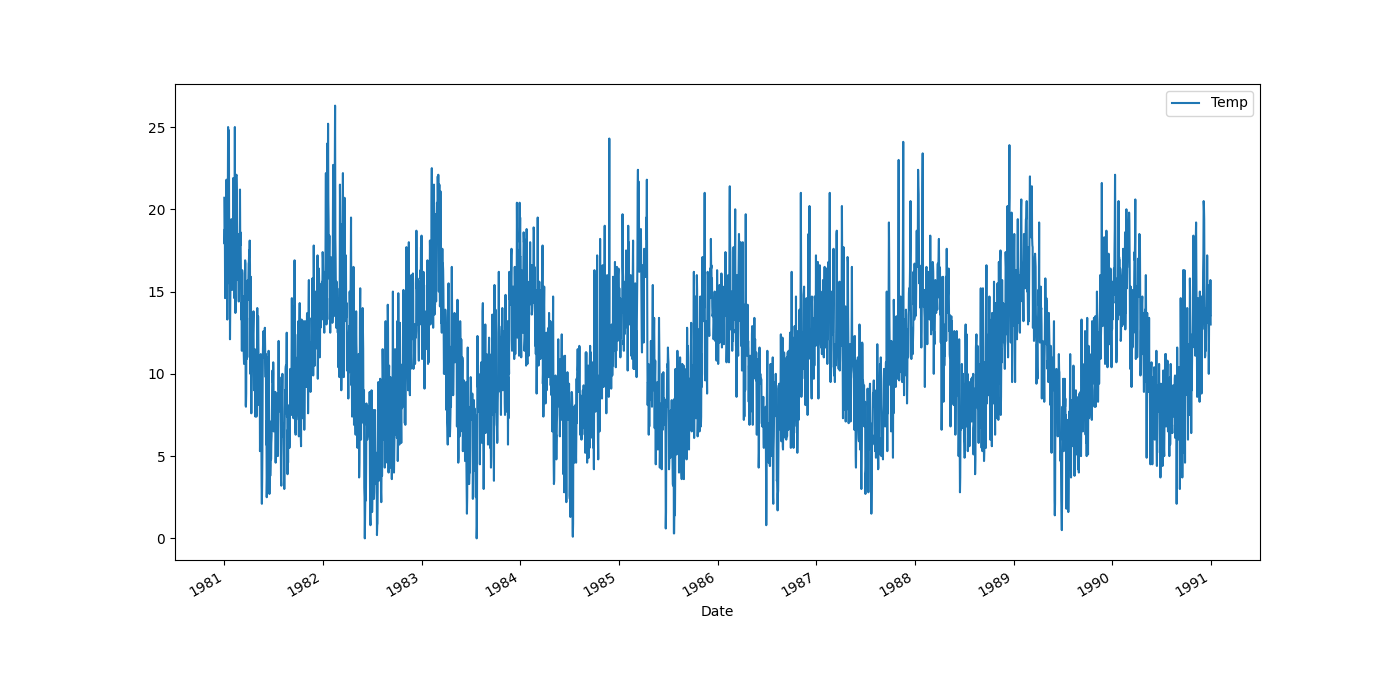
\includegraphics[width=\textwidth]{figures/Ass1/Ass1_D1_raw_signal.png}
    \end{minipage}
    \caption{The raw signal of the first dataset.}
    \label{fig:Ass1_D1_raw_signal}
\end{figure}

\begin{figure}[H]
    \centering
    \begin{minipage}[b]{1\textwidth}
        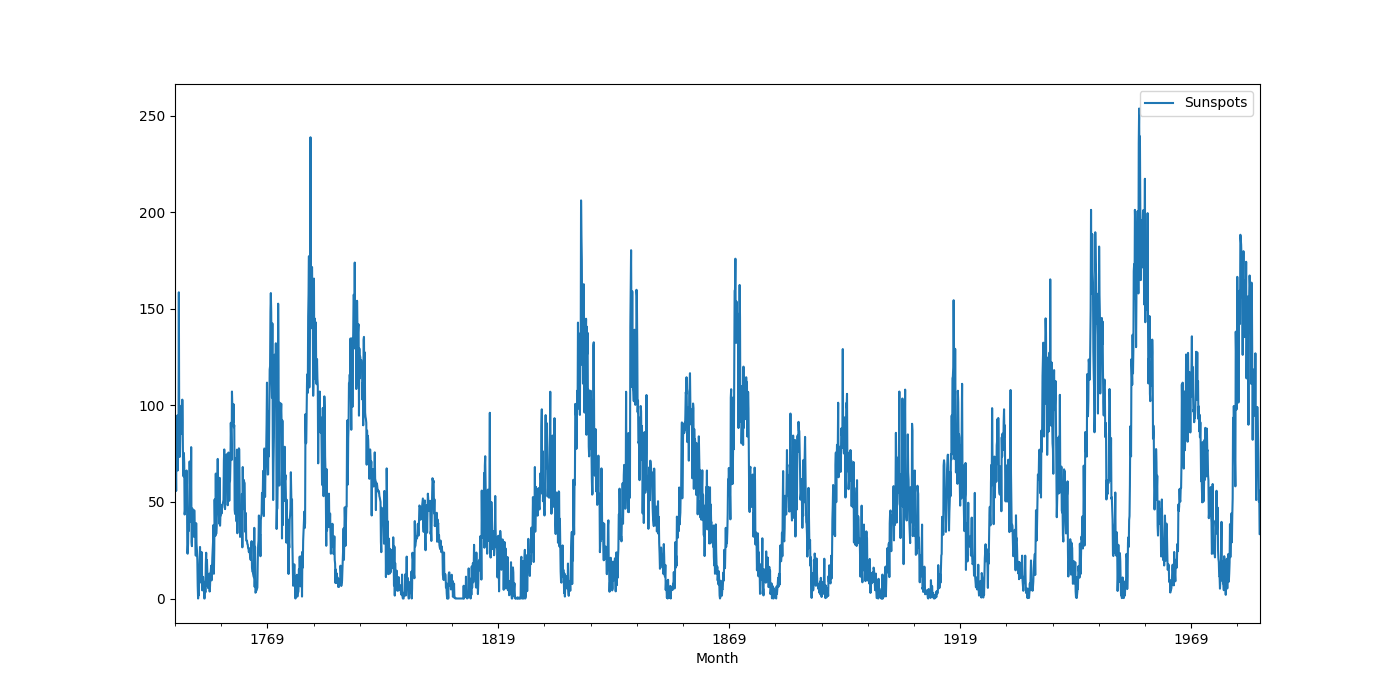
\includegraphics[width=\textwidth]{figures/Ass1/Ass1_D2_raw_signal.png}
    \end{minipage}
    \caption{The raw signal of the second dataset.}
    \label{fig:Ass1_D2_raw_signal}
\end{figure}

\begin{figure}[H]
    \centering
    \begin{minipage}[b]{1\textwidth}
        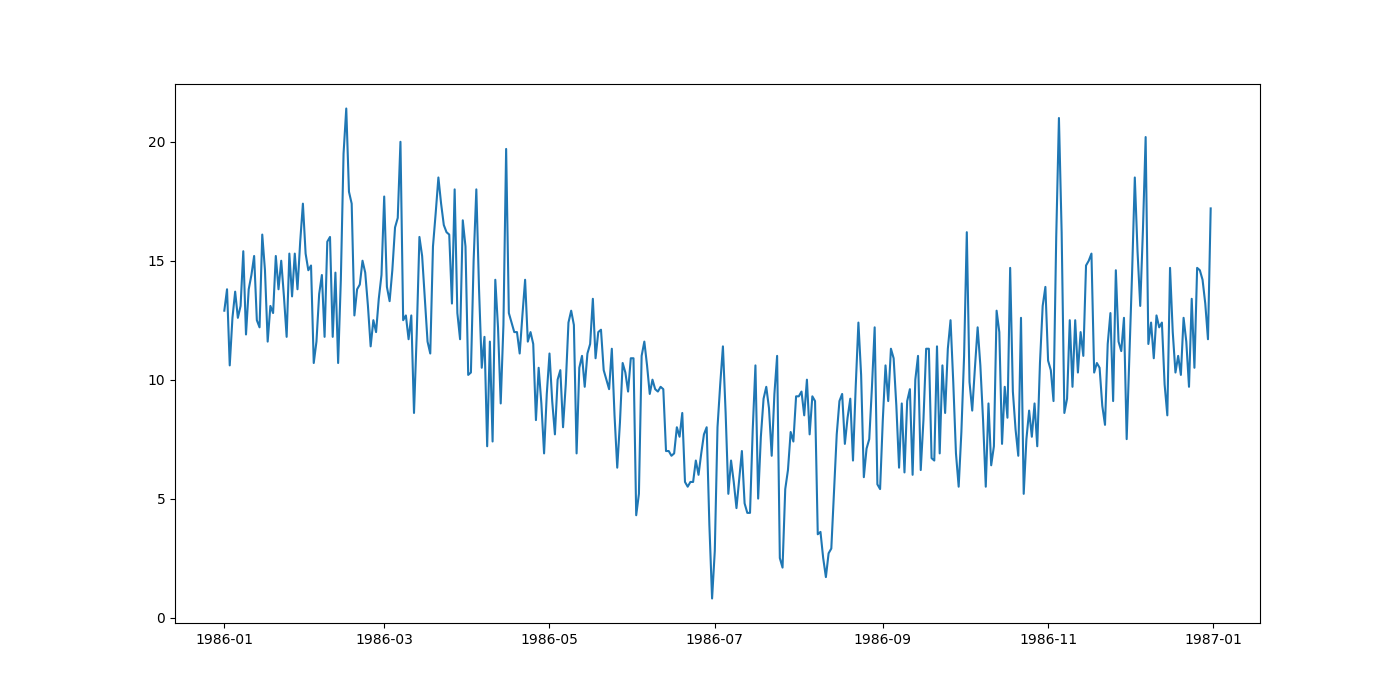
\includegraphics[width=\textwidth]{figures/Ass1/Ass1_D1_raw_signal_1986.png}
    \end{minipage}
    \caption{Visualizing a short period of the first dataset.}
    \label{fig:Ass1_D1_raw_signal_1986}
\end{figure}


\begin{figure}[H]
    \centering
    \begin{minipage}[b]{1\textwidth}
        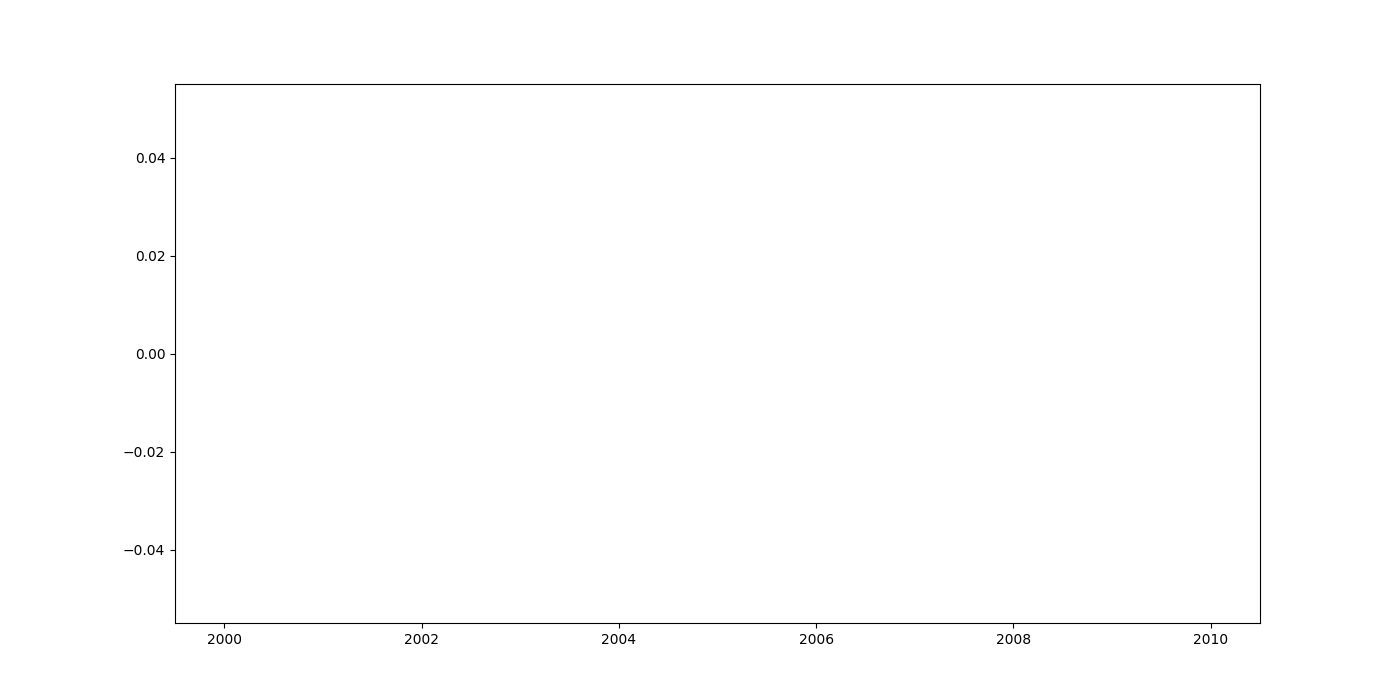
\includegraphics[width=\textwidth]{figures/Ass1/Ass1_D2_raw_signal_1990.png}
    \end{minipage}
    \caption{Visualizing a short period of the second dataset.}
    \label{fig:Ass1_D2_raw_signal_1990}
\end{figure}

\textit{For intuition, Table \ref{tab:Ass1_D1_raw_signal} to  \ref{tab:Ass1_D2_raw_signal_summary_statistics} show the top raw of two datasets along with the descriptive statistics of two time-series datasets.}


\begin{table}[H]
 \centering
\caption{The first five rows of the raw signal in the first dataset.}
\label{tab:Ass1_D1_raw_signal}
\begin{tabular}{lr}
\toprule
{} &  Temp \\
Date       &       \\
\midrule
1981-01-01 &  20.7 \\
1981-01-02 &  17.9 \\
1981-01-03 &  18.8 \\
1981-01-04 &  14.6 \\
1981-01-05 &  15.8 \\
1981-01-06 &  15.8 \\
1981-01-07 &  15.8 \\
\bottomrule
\end{tabular}

\end{table}

\begin{table}[H]
 \centering
\caption{The descriptive statistics of the first dataset.}
\label{tab:Ass1_D1_raw_signal_summary_statistics}
\begin{tabular}{lr}
\toprule
{} &         Temp \\
\midrule
count &  3650.000000 \\
mean  &    11.177753 \\
std   &     4.071837 \\
min   &     0.000000 \\
25\%   &     8.300000 \\
50\%   &    11.000000 \\
75\%   &    14.000000 \\
max   &    26.300000 \\
\bottomrule
\end{tabular}

\end{table}

\begin{table}[H]
 \centering
\caption{The first five rows of the raw signal in the second dataset.}
\label{tab:Ass1_D2_raw_signal}
\begin{tabular}{lr}
\toprule
{} &  Sunspots \\
Month      &           \\
\midrule
1749-01-01 &      58.0 \\
1749-02-01 &      62.6 \\
1749-03-01 &      70.0 \\
1749-04-01 &      55.7 \\
1749-05-01 &      85.0 \\
\bottomrule
\end{tabular}

\end{table}

\begin{table}[H]
 \centering
\caption{The descriptive statistics of the second dataset.} \label{tab:Ass1_D2_raw_signal_summary_statistics}
\begin{tabular}{lr}
\toprule
{} &     Sunspots \\
\midrule
count &  2820.000000 \\
mean  &    51.265957 \\
std   &    43.448971 \\
min   &     0.000000 \\
25\%   &    15.700000 \\
50\%   &    42.000000 \\
75\%   &    74.925000 \\
max   &   253.800000 \\
\bottomrule
\end{tabular}

\end{table}






\textit{For decomposing the time series, the below methods used:}
    \begin{enumerate}
    \item \textit{Seasonal\_decompose (Figure
        \ref{fig:Ass1_D1_seasonal_decompose} and \ref{fig:Ass1_D2_seasonal_decompose})}
        
    \item \textit{STL (Figure
        \ref{fig:Ass1_D1_STL} and \ref{fig:Ass1_D2_STL})}
        
    \item \textit{Linear Regression method (Figure
        \ref{fig:Ass1_D1_LinearRegression_diff} and \ref{fig:Ass1_D2_LinearRegression_diff})}
        
    \item \textit{Difference method (Figure
        \ref{fig:Ass1_D1_one_diff} and \ref{fig:Ass1_D2_one_diff})}
        
    \item \textit{Fitting a polynomial (Figure
        \ref{fig:Ass1_D1_fiting_polynomial} and \ref{fig:Ass1_D2_fiting_polynomial})}
        
    \item \textit{Moving Average window (Figure
        \ref{fig:Ass1_D1_Moving_Avrage} and \ref{fig:Ass1_D2_Moving_Avrage})}

    \end{enumerate}

\textit{\newline \newline Some mentioned methods used only for extracting only one type of component (trend or seasonality), while others like STL 
and Seasonal\_decompose provided all three parts. Table \ref{tab:Ass1_comparing_methods} compares these methods together.}

\textit{Also, there are two models for the reconstruction of time series, Additive and Multiplicative Model. In this assignment, the additive model was only used because the multiplicative model is not appropriate for zero and negative values.}

\begin{table}[H]
\centering
\caption{Comparing the implemented methods.}
\label{tab:Ass1_comparing_methods}
\begin{tabular}{@{}lccc@{}}
\toprule
                    & \begin{tabular}[c]{@{}c@{}}Trend \\ component\end{tabular} & \begin{tabular}[c]{@{}c@{}}Seasonal \\ component\end{tabular} & \begin{tabular}[c]{@{}c@{}}Residual \\ component\end{tabular} \\ \midrule
Seasonal\_decompose & \checkmark                                  & \checkmark                                     & \checkmark                                     \\ \midrule
STL                 & \checkmark                                  & \checkmark                                     & \checkmark                                     \\ \midrule
Linear Regression   & \checkmark                                  & -                                                             & -                                                             \\ \midrule
Difference          & -                                                          & \checkmark                                     & -                                                             \\ \midrule
Moving average      & \checkmark                                  & -                                                             & -                                                             \\ \bottomrule
\end{tabular}

\end{table}


\textit{For finding the seasonal component, we need to find the period of the time series. For doing this, the resampling method was used to smooth the plots of two datasets. Figures \ref{fig:Ass1_D1_resample} and \ref{fig:Ass1_D2_resample} indicate the smooth version of the two datasets. }

\begin{figure}[H]
    \centering
    \begin{minipage}[b]{1\textwidth}
        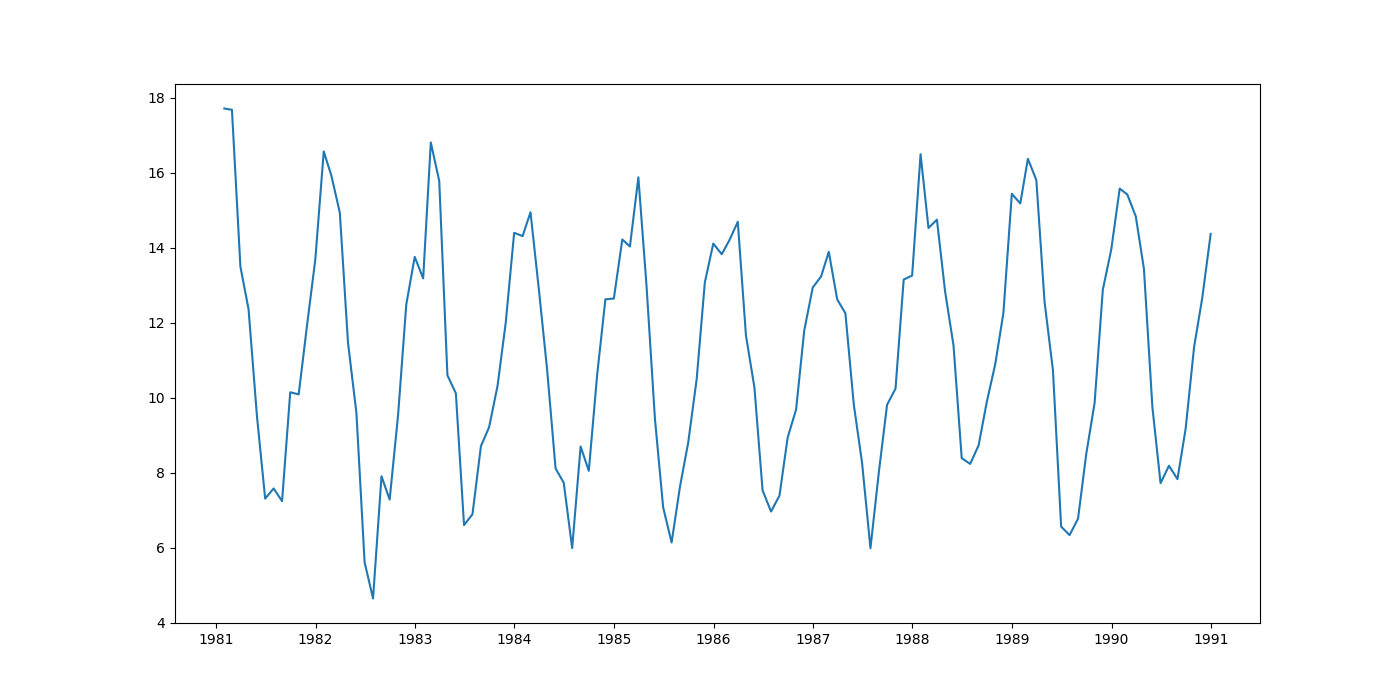
\includegraphics[width=\textwidth]{figures/Ass1/Ass1_D1_resample.png}
    \end{minipage}
    \caption{Resampling plot of the first dataset. The period of this dataset is 365 samples/cycle. }
    \label{fig:Ass1_D1_resample}
\end{figure}

\begin{figure}[H]
    \centering
    \begin{minipage}[b]{1\textwidth}
        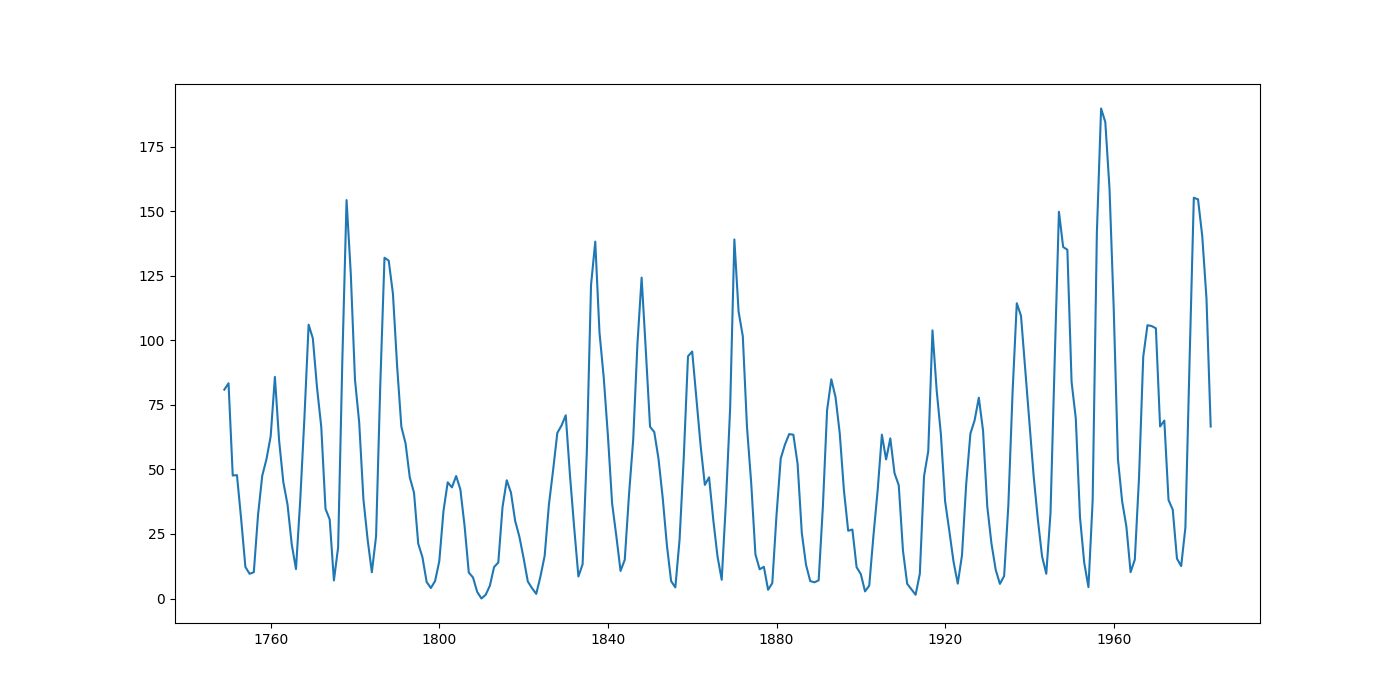
\includegraphics[width=\textwidth]{figures/Ass1/Ass1_D2_resample.png}
    \end{minipage}
    \caption{Resampling plot of the second dataset. The period of this dataset is 130 samples/cycle.}
    \label{fig:Ass1_D2_resample}
\end{figure}


\textit{Furthermore, the period of the time-series data can calculate by \gls{ACF} (figures \ref{fig:Ass1_D1_PACF_ACF_series} and \ref{fig:Ass1_D2_PACF_ACF_series}). This plot has an oscillation, indicative of a seasonal series and the peaks occurred at each period. }

\begin{figure}[H]
    \centering
    \begin{minipage}[b]{1\textwidth}
        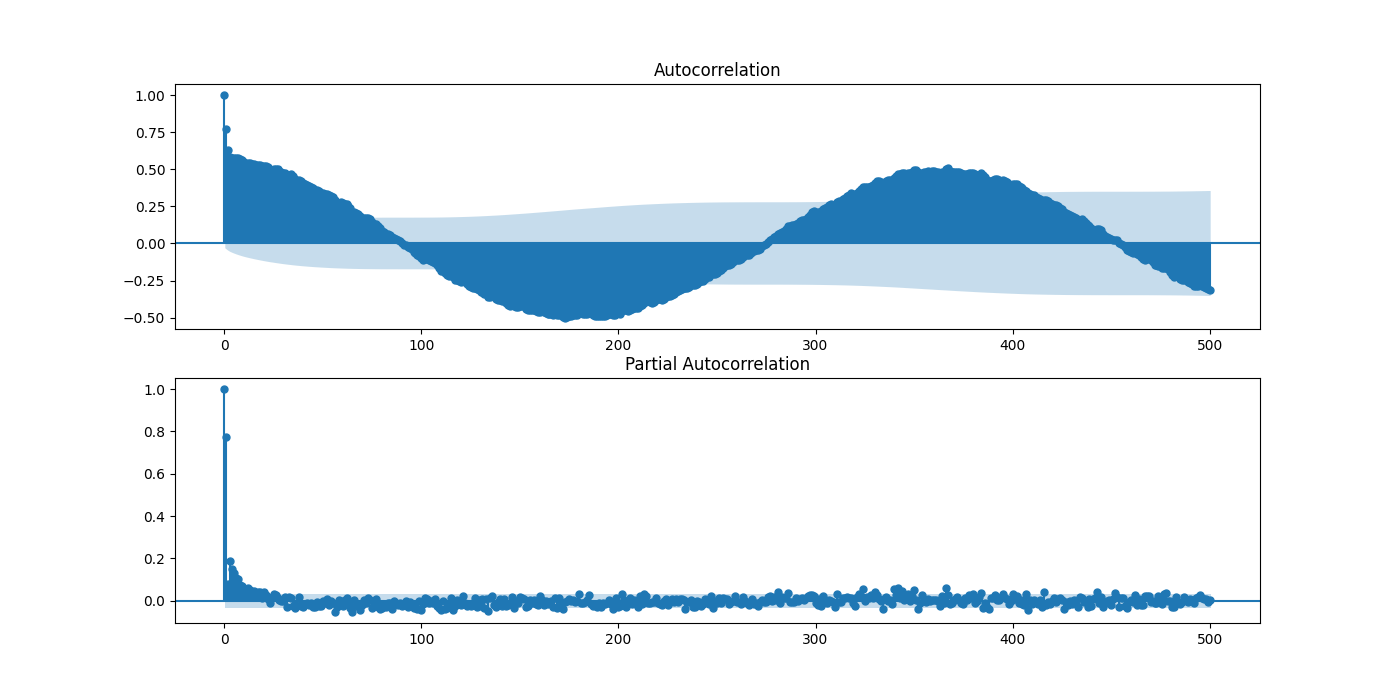
\includegraphics[width=\textwidth]{figures/Ass1/Ass1_D1_PACF_ACF_series.png}
    \end{minipage}
    \caption{The \gls{ACF} and \gls{PACF} of the first dataset. The peaks occur at the lag of 365 that means the period is 365 samples/cycle.}
    \label{fig:Ass1_D1_PACF_ACF_series}
\end{figure}

\begin{figure}[H]
    \centering
    \begin{minipage}[b]{1\textwidth}
        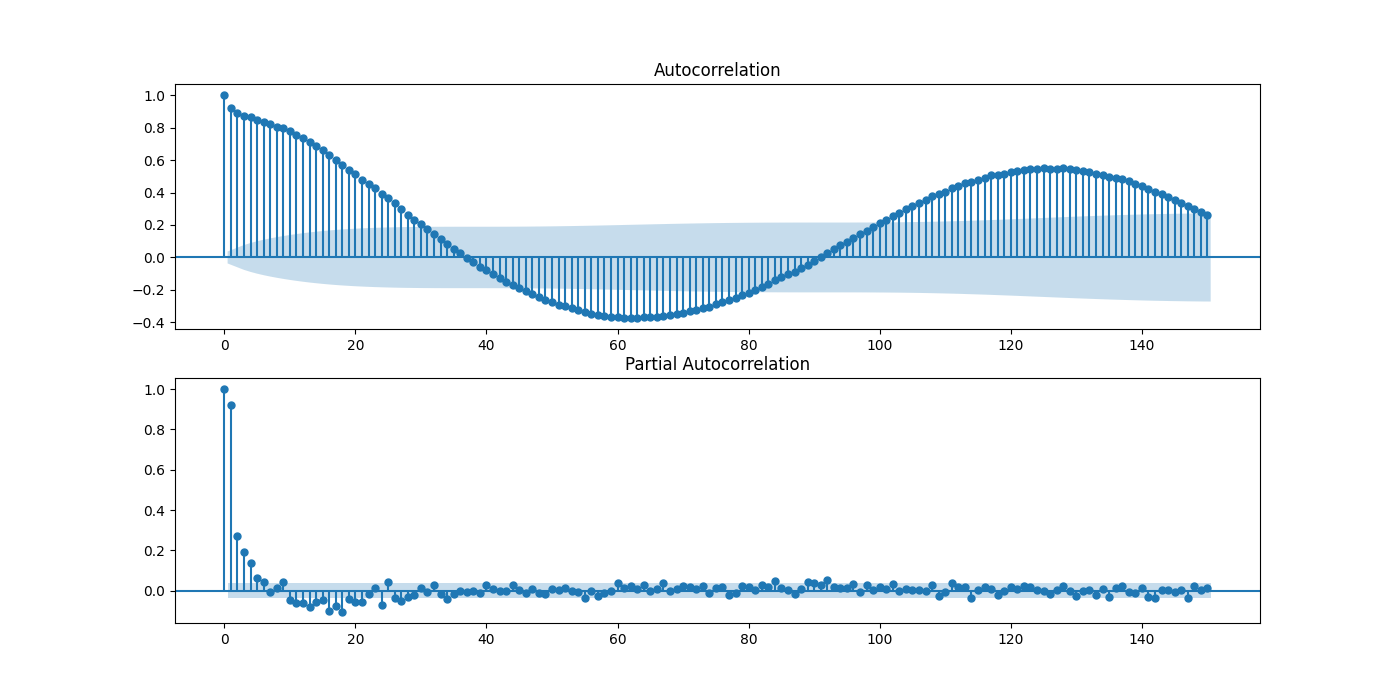
\includegraphics[width=\textwidth]{figures/Ass1/Ass1_D2_PACF_ACF_series.png}
    \end{minipage}
    \caption{The \gls{ACF} and \gls{PACF} of the second dataset. The peaks occur at the lag of 130 that means the period is 130 samples/cycle.}
    \label{fig:Ass1_D2_PACF_ACF_series}
\end{figure}


\begin{figure}[H]
    \centering
    \begin{minipage}[b]{1\textwidth}
        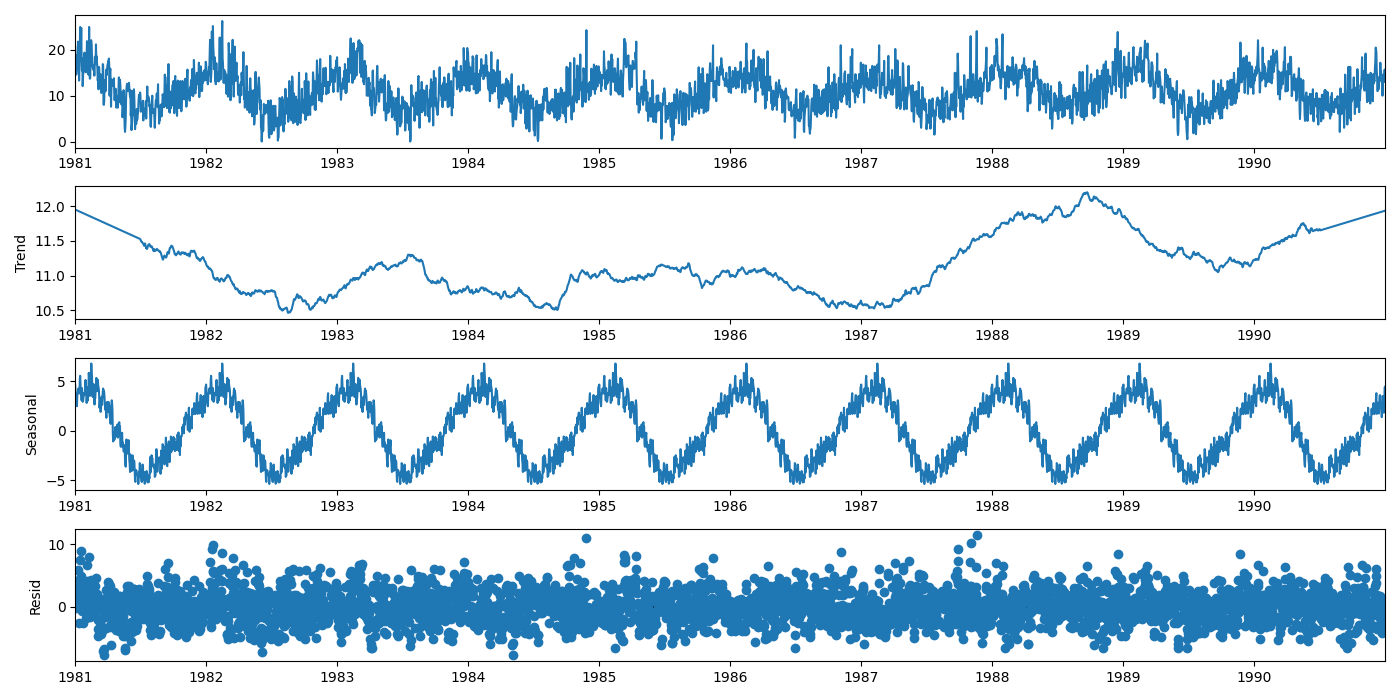
\includegraphics[width=\textwidth]{figures/Ass1/Ass1_D1_seasonal_decompose.png}
    \end{minipage}
    \caption{Decomposition of the first dataset by seasonal\_decompose method}
    \label{fig:Ass1_D1_seasonal_decompose}
\end{figure}

\begin{figure}[H]
    \centering
    \begin{minipage}[b]{1\textwidth}
        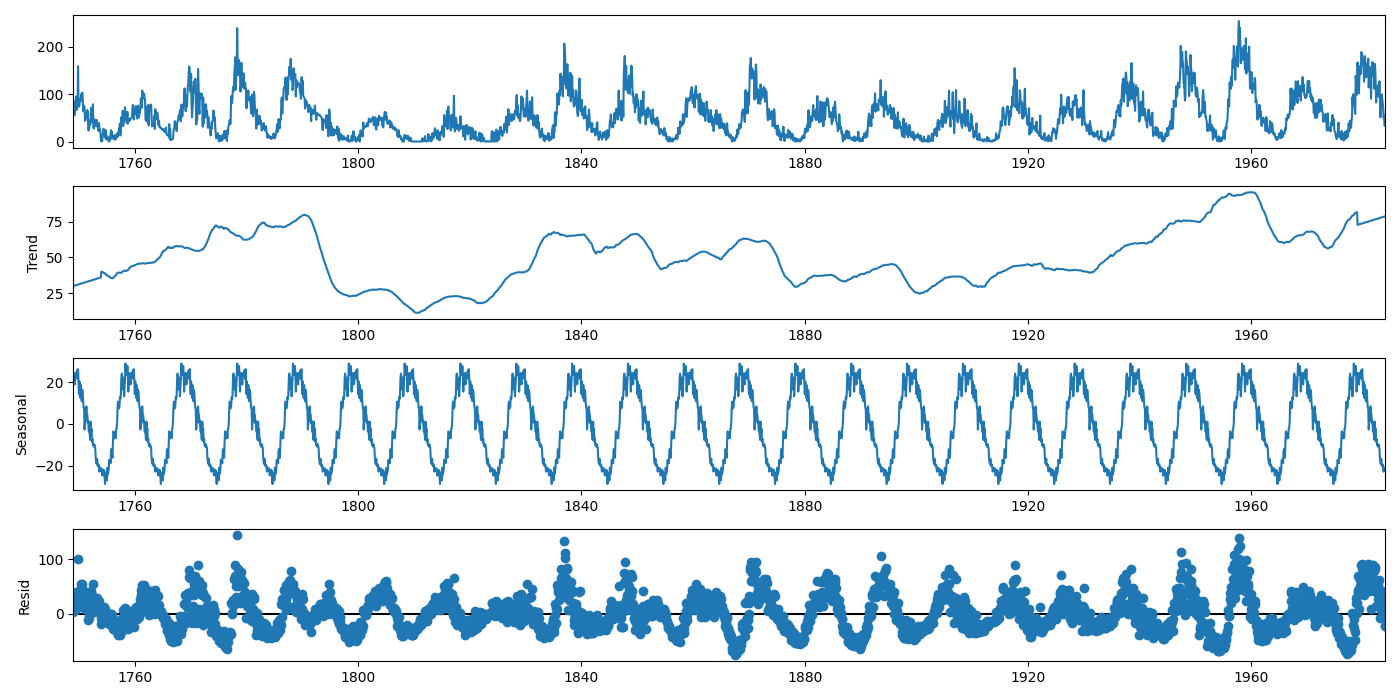
\includegraphics[width=\textwidth]{figures/Ass1/Ass1_D2_seasonal_decompose.png}
    \end{minipage}
    \caption{Decomposition of the second dataset by seasonal\_decompose method}
    \label{fig:Ass1_D2_seasonal_decompose}
\end{figure}

\begin{figure}[H]
    \centering
    \begin{minipage}[b]{1\textwidth}
        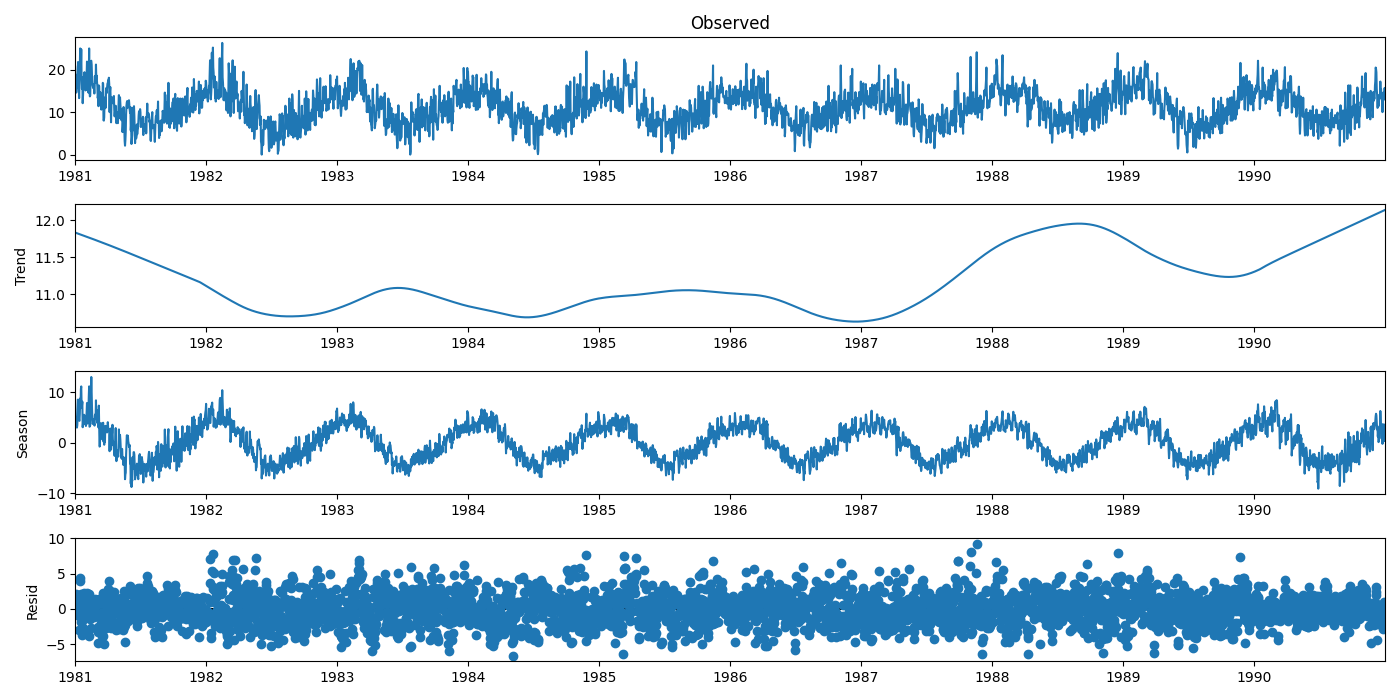
\includegraphics[width=\textwidth]{figures/Ass1/Ass1_D1_STL.png}
    \end{minipage}
    \caption{Decomposition of the first dataset by STL method}
    \label{fig:Ass1_D1_STL}
\end{figure}

\begin{figure}[H]
    \centering
    \begin{minipage}[b]{1\textwidth}
        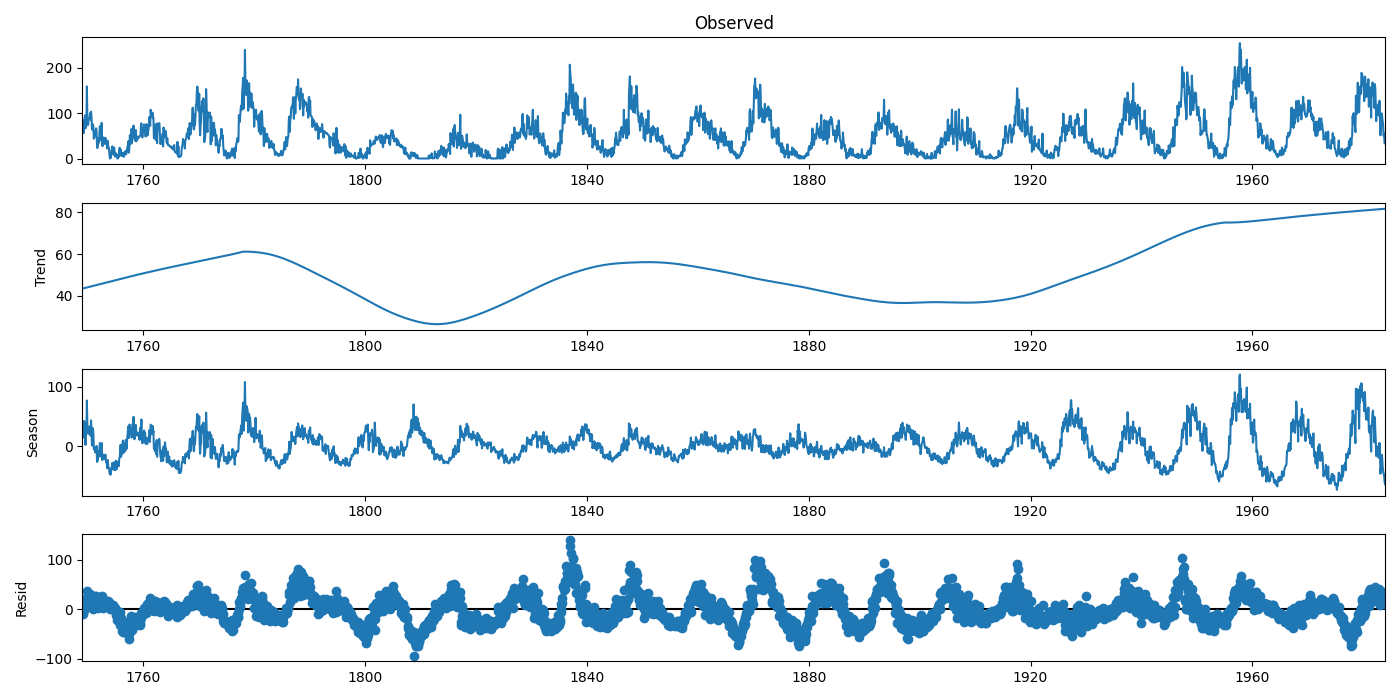
\includegraphics[width=\textwidth]{figures/Ass1/Ass1_D2_STL.png}
    \end{minipage}
    \caption{Decomposition of the second dataset by STL method}
    \label{fig:Ass1_D2_STL}
\end{figure}

\begin{figure}[H]
    \centering
    \begin{minipage}[b]{1\textwidth}
        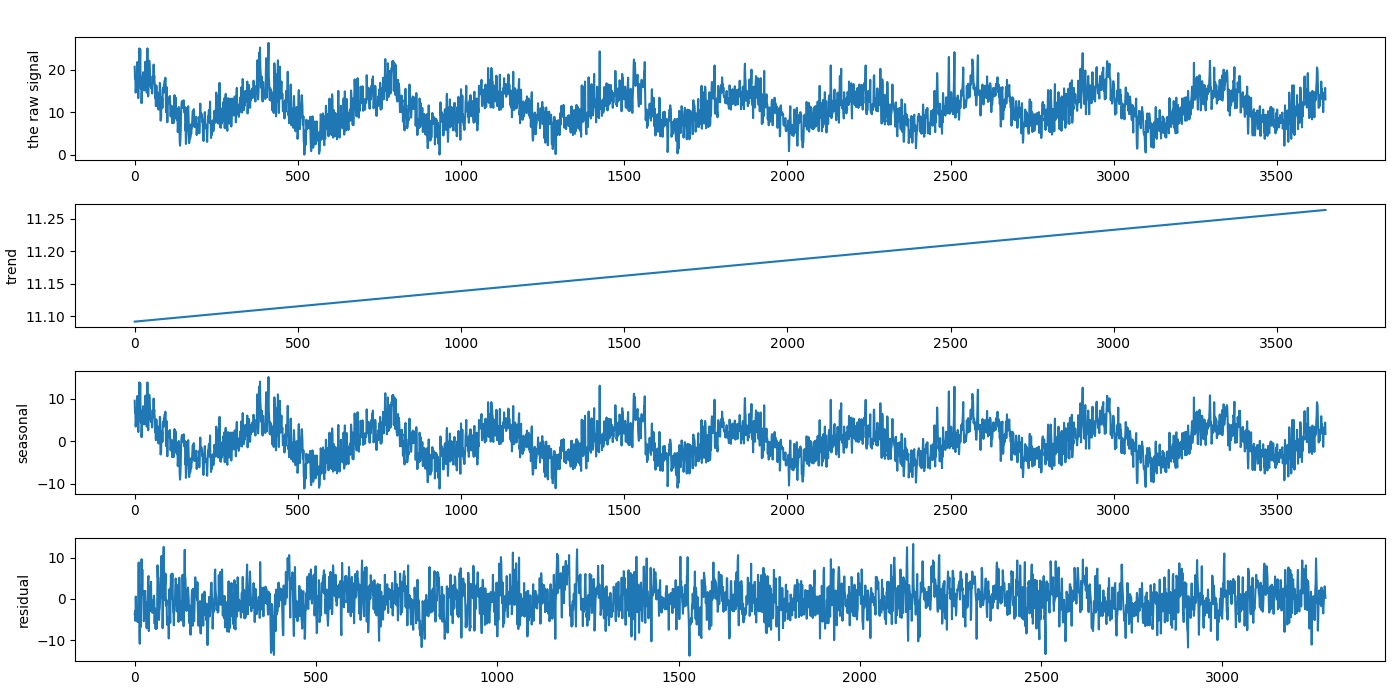
\includegraphics[width=\textwidth]{figures/Ass1/Ass1_D1_LinearRegression_diff.png}
    \end{minipage}
    \caption{Decomposition of the first dataset by Linear Regression and difference method.}
    \label{fig:Ass1_D1_LinearRegression_diff}
\end{figure}

\begin{figure}[H]
    \centering
    \begin{minipage}[b]{1\textwidth}
        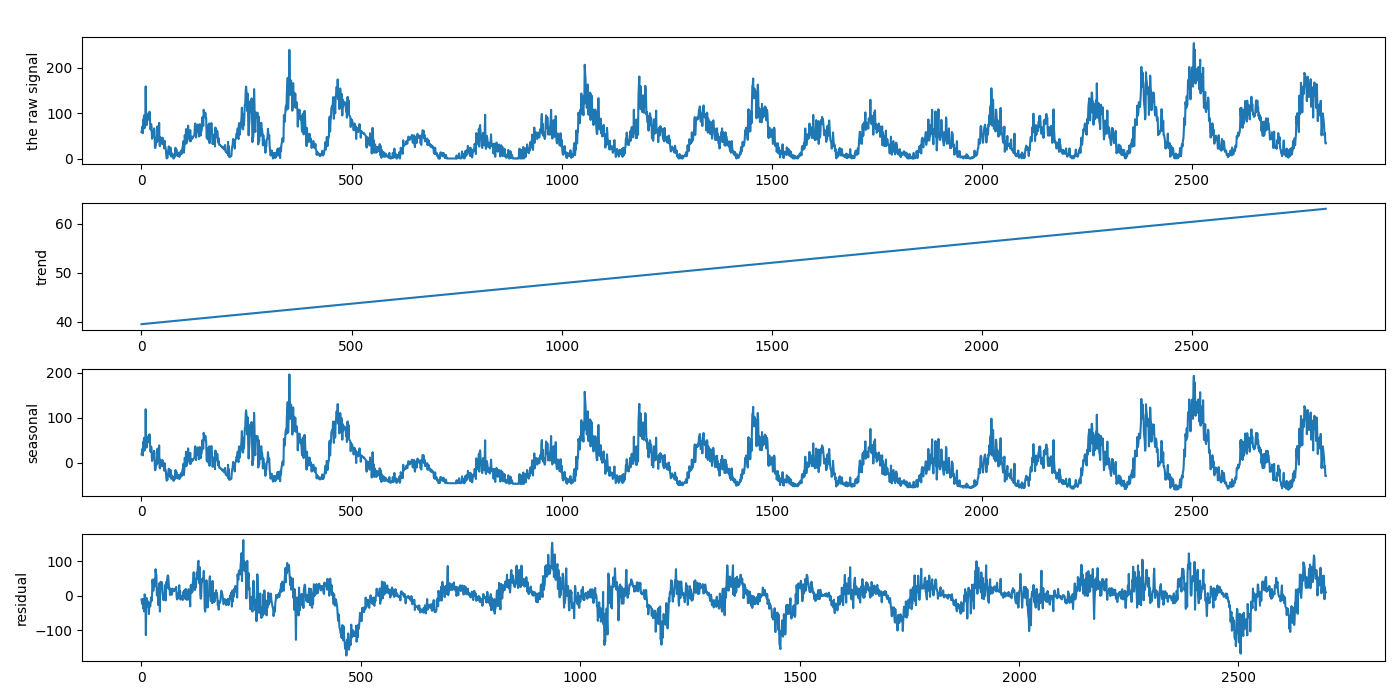
\includegraphics[width=\textwidth]{figures/Ass1/Ass1_D2_LinearRegression_diff.png}
    \end{minipage}
    \caption{Decomposition of the second dataset by Linear Regression and difference method.}
    \label{fig:Ass1_D2_LinearRegression_diff}
\end{figure}

\begin{figure}[H]
    \centering
    \begin{minipage}[b]{1\textwidth}
        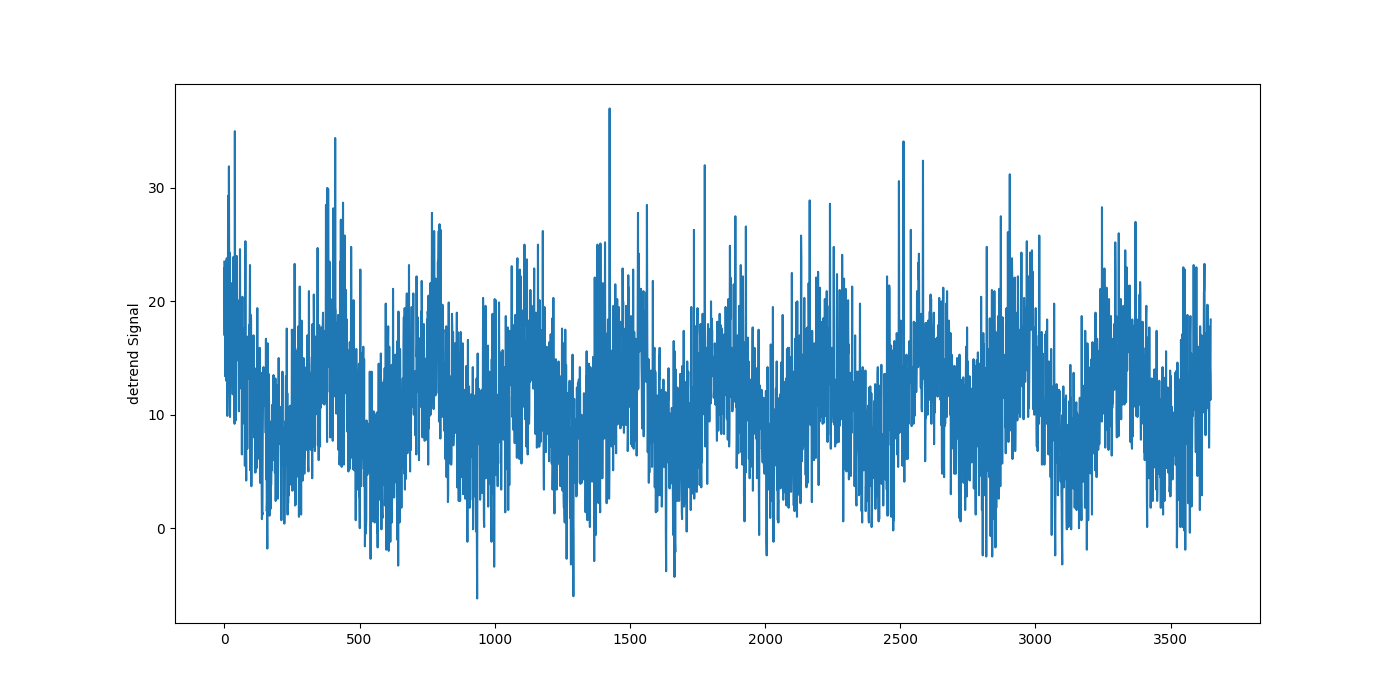
\includegraphics[width=\textwidth]{figures/Ass1/Ass1_D1_one_diff.png}
    \end{minipage}
    \caption{Detrending of the first dataset by the first-order differencing.}
    \label{fig:Ass1_D1_one_diff}
\end{figure}

\begin{figure}[H]
    \centering
    \begin{minipage}[b]{1\textwidth}
        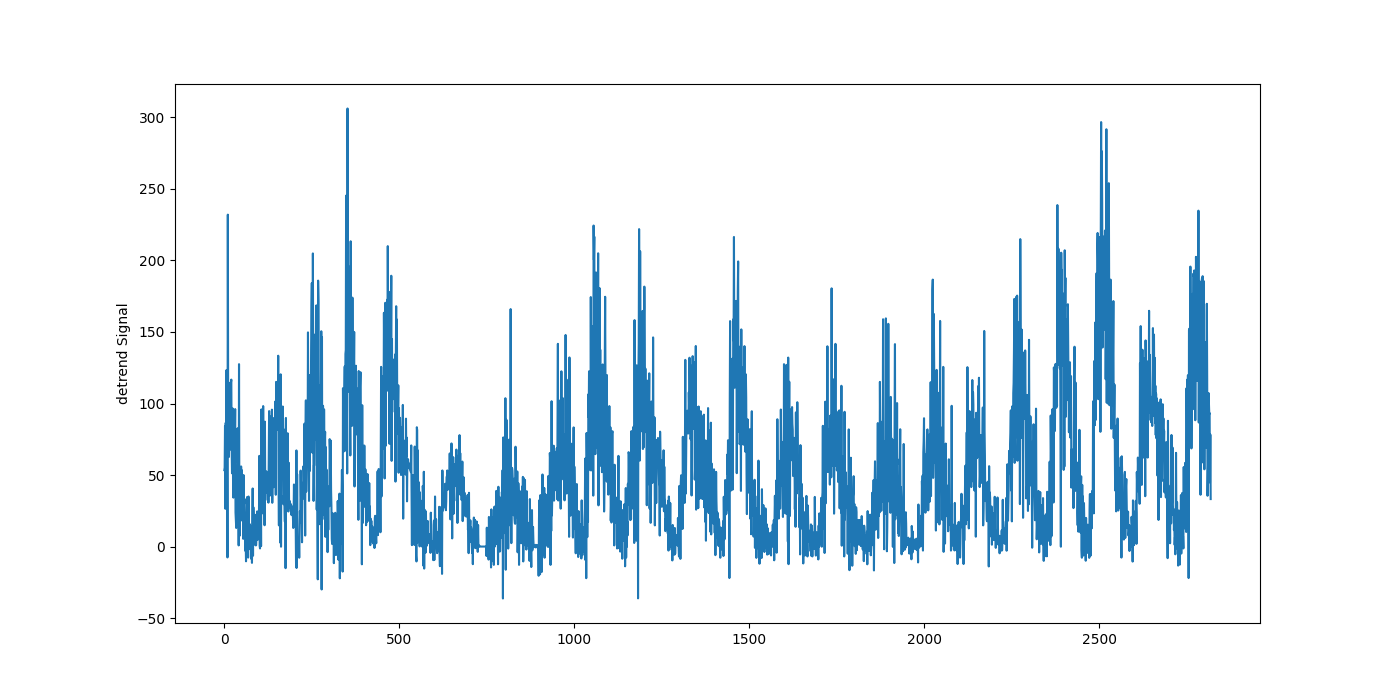
\includegraphics[width=\textwidth]{figures/Ass1/Ass1_D2_one_diff.png}
    \end{minipage}
    \caption{Detrending of the second dataset by the first-order differencing.}
    \label{fig:Ass1_D2_one_diff}
\end{figure}

\begin{figure}[H]
    \centering
    \begin{minipage}[b]{1\textwidth}
        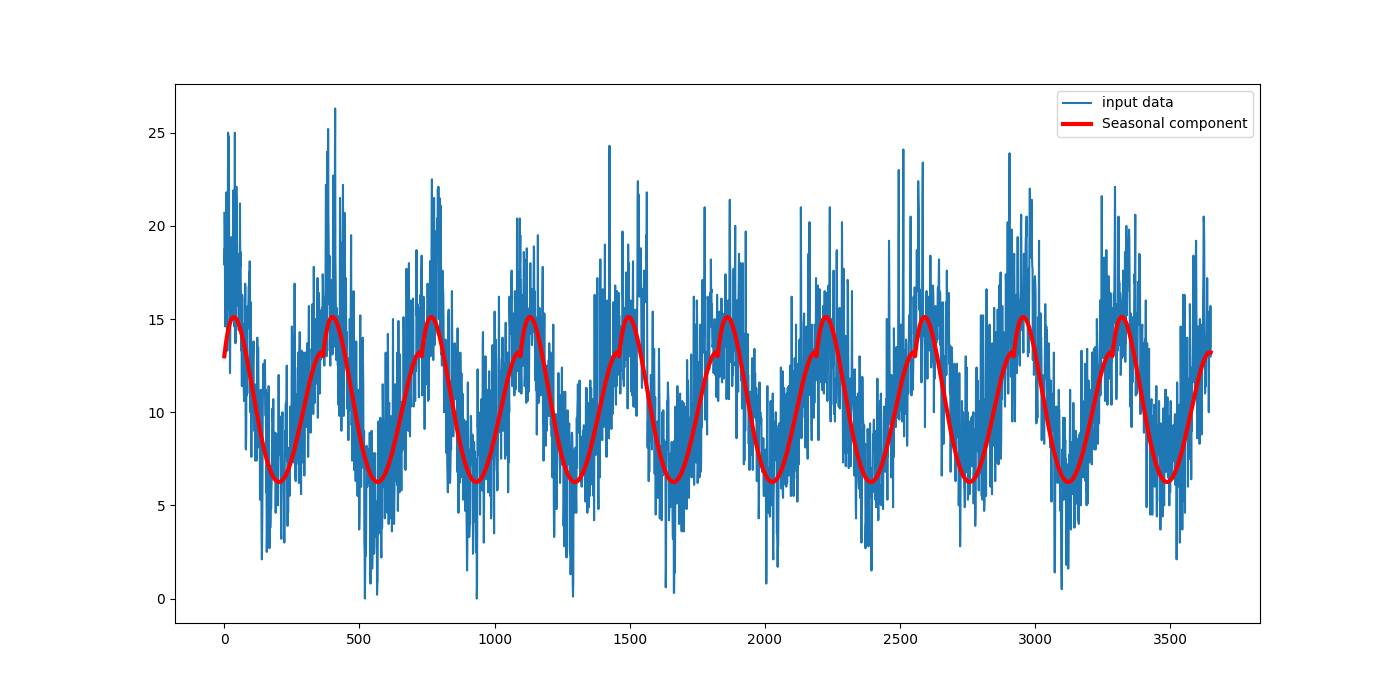
\includegraphics[width=\textwidth]{figures/Ass1/Ass1_D1_fiting_polynomial.png}
    \end{minipage}
    \caption{Seasonal component of the first dataset by fitting a polynomial (Degree of the polynomial is 4).}
    \label{fig:Ass1_D1_fiting_polynomial}
\end{figure}

\begin{figure}[H]
    \centering
    \begin{minipage}[b]{1\textwidth}
        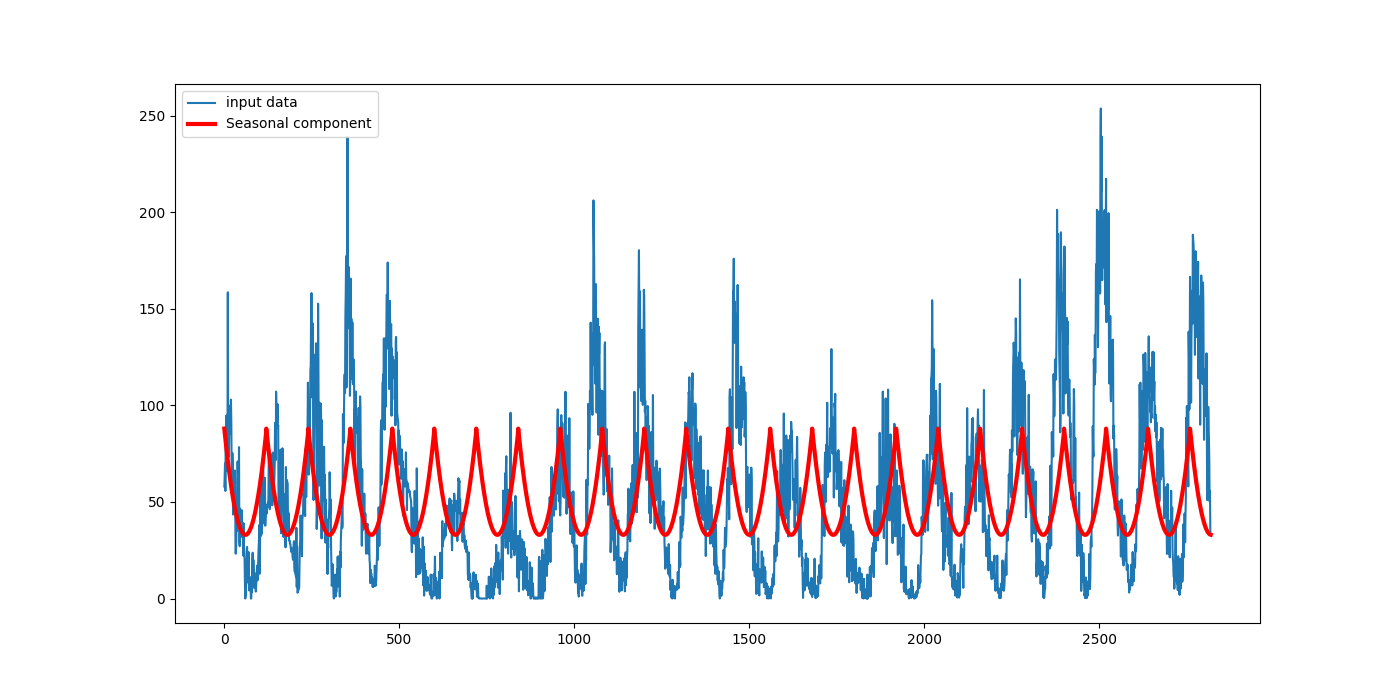
\includegraphics[width=\textwidth]{figures/Ass1/Ass1_D2_fiting_polynomial.png}
    \end{minipage}
    \caption{Seasonal component of the second dataset by fitting a polynomial (Degree of the polynomial is 2).}
    \label{fig:Ass1_D2_fiting_polynomial}
\end{figure}

\begin{figure}[H]
    \centering
    \begin{minipage}[b]{1\textwidth}
        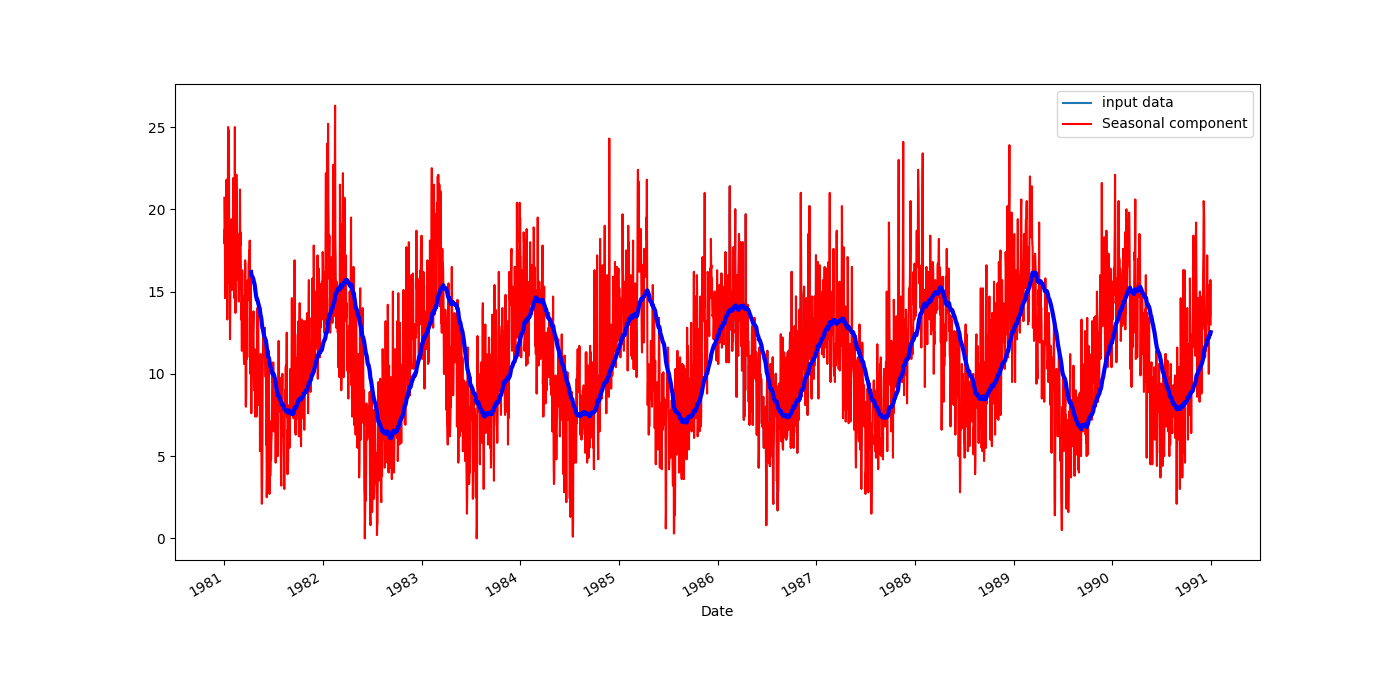
\includegraphics[width=\textwidth]{figures/Ass1/Ass1_D1_Moving_Avrage.png}
    \end{minipage}
    \caption{Seasonal component of the first dataset by Moving Average. The size of the window was set to 100.}
    \label{fig:Ass1_D1_Moving_Avrage}
\end{figure}

\begin{figure}[H]
    \centering
    \begin{minipage}[b]{1\textwidth}
        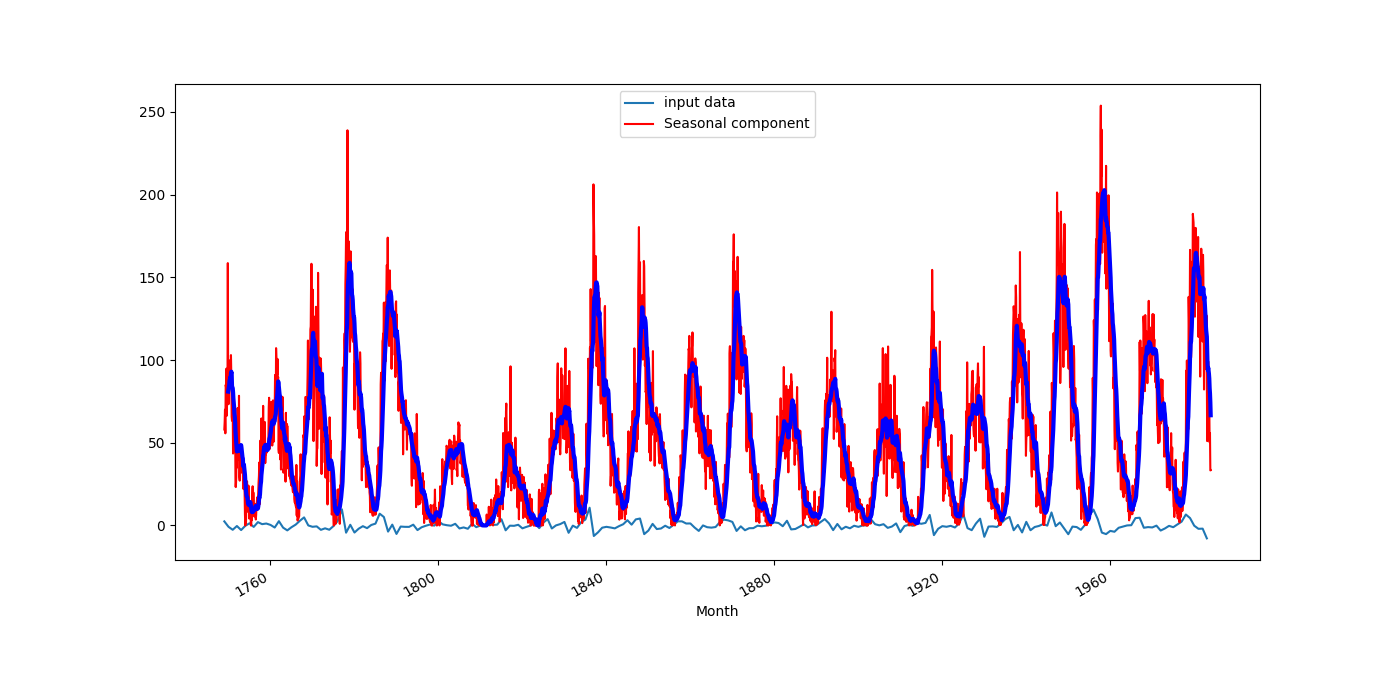
\includegraphics[width=\textwidth]{figures/Ass1/Ass1_D2_Moving_Avrage.png}
    \end{minipage}
    \caption{Seasonal component of the second dataset by Moving Average. The size of the window was set to 12.  }
    \label{fig:Ass1_D2_Moving_Avrage}
\end{figure}



